% Options for packages loaded elsewhere
\PassOptionsToPackage{unicode}{hyperref}
\PassOptionsToPackage{hyphens}{url}
\PassOptionsToPackage{dvipsnames,svgnames,x11names}{xcolor}
\documentclass[
  10pt,
]{article}
\usepackage{xcolor}
\usepackage[margin=1in]{geometry}
\usepackage{amsmath,amssymb}
\setcounter{secnumdepth}{-\maxdimen} % remove section numbering
\usepackage{iftex}
\ifPDFTeX
  \usepackage[T1]{fontenc}
  \usepackage[utf8]{inputenc}
  \usepackage{textcomp} % provide euro and other symbols
\else % if luatex or xetex
  \usepackage{unicode-math} % this also loads fontspec
  \defaultfontfeatures{Scale=MatchLowercase}
  \defaultfontfeatures[\rmfamily]{Ligatures=TeX,Scale=1}
\fi
\usepackage{lmodern}
\ifPDFTeX\else
  % xetex/luatex font selection
\fi
% Use upquote if available, for straight quotes in verbatim environments
\IfFileExists{upquote.sty}{\usepackage{upquote}}{}
\IfFileExists{microtype.sty}{% use microtype if available
  \usepackage[]{microtype}
  \UseMicrotypeSet[protrusion]{basicmath} % disable protrusion for tt fonts
}{}
\makeatletter
\@ifundefined{KOMAClassName}{% if non-KOMA class
  \IfFileExists{parskip.sty}{%
    \usepackage{parskip}
  }{% else
    \setlength{\parindent}{0pt}
    \setlength{\parskip}{6pt plus 2pt minus 1pt}}
}{% if KOMA class
  \KOMAoptions{parskip=half}}
\makeatother
\usepackage{longtable,booktabs,array}
\usepackage{calc} % for calculating minipage widths
% Correct order of tables after \paragraph or \subparagraph
\usepackage{etoolbox}
\makeatletter
\patchcmd\longtable{\par}{\if@noskipsec\mbox{}\fi\par}{}{}
\makeatother
% Allow footnotes in longtable head/foot
\IfFileExists{footnotehyper.sty}{\usepackage{footnotehyper}}{\usepackage{footnote}}
\makesavenoteenv{longtable}
\usepackage{graphicx}
\makeatletter
\newsavebox\pandoc@box
\newcommand*\pandocbounded[1]{% scales image to fit in text height/width
  \sbox\pandoc@box{#1}%
  \Gscale@div\@tempa{\textheight}{\dimexpr\ht\pandoc@box+\dp\pandoc@box\relax}%
  \Gscale@div\@tempb{\linewidth}{\wd\pandoc@box}%
  \ifdim\@tempb\p@<\@tempa\p@\let\@tempa\@tempb\fi% select the smaller of both
  \ifdim\@tempa\p@<\p@\scalebox{\@tempa}{\usebox\pandoc@box}%
  \else\usebox{\pandoc@box}%
  \fi%
}
% Set default figure placement to htbp
\def\fps@figure{htbp}
\makeatother
\setlength{\emergencystretch}{3em} % prevent overfull lines
\providecommand{\tightlist}{%
  \setlength{\itemsep}{0pt}\setlength{\parskip}{0pt}}
\usepackage[]{natbib}
\bibliographystyle{plainnat}
% Extra packages for the manuscript build. Loaded after the pandoc default template's own packages.
\usepackage{longtable,booktabs,array}
\usepackage{etoolbox}
\usepackage{caption}
\usepackage{float}

% Tables in this paper are wide (up to seven columns); longtable gets a smaller font so they fit the text block.
\AtBeginEnvironment{longtable}{\small}

% Figures are rendered at column width and keep their aspect ratio; the PNGs are 2x for print.
\setkeys{Gin}{width=0.85\linewidth,height=0.32\textheight,keepaspectratio}
\captionsetup{font=small,labelfont=bf}

% Inline \texttt{} paths cannot wrap; let the paragraph stretch instead of running into the margin.
\setlength{\emergencystretch}{3em}

% Pages end where the content ends: a float plus a long table fragment should not be stretched to the full measure.
\raggedbottom
\usepackage{bookmark}
\IfFileExists{xurl.sty}{\usepackage{xurl}}{} % add URL line breaks if available
\urlstyle{same}
\hypersetup{
  pdftitle={Deterministic Diagnosis, Generative Prose: Separating Verdict from Narrative in Industrial Fault Reporting},
  colorlinks=true,
  linkcolor={blue},
  filecolor={Maroon},
  citecolor={Blue},
  urlcolor={blue},
  pdfcreator={LaTeX via pandoc}}

\title{Deterministic Diagnosis, Generative Prose: Separating Verdict
from Narrative in Industrial Fault Reporting}
\author{}
\date{17 November 2026}

\begin{document}
\maketitle

\textbf{Journal manuscript (TEP-FP), 17 November 2026.} Single-column
submission format. The paper reports the \textbf{Version B} framing
signed on 2026-11-17: the preference study is reported descriptively and
supports no ordering. Every number below is re-derived from a committed,
SHA-256-hashed artefact in \texttt{docs/\allowbreak{}reports/\allowbreak{}evidence/\allowbreak{}} (Appendix A),
and figures are rendered from stored JSON rather than redrawn.
Corresponding author, affiliations and funding are completed at
submission.

\begin{center}\rule{0.5\linewidth}{0.5pt}\end{center}

\subsection{Abstract}\label{abstract}

Industrial fault reports have two jobs: to be right and to be readable.
We separate them. In the system studied here the verdict, fault
identity, severity and confidence are computed deterministically from
the evidence store, and a 2-billion-parameter vision-language adapter,
fine-tuned with LoRA, writes only the prose and handles follow-up
dialogue. On 3,168 held-out events from a simulated chemical plant the
adapter stays inside a pre-registered 2 \% numeric-fidelity budget (40
defective reports, 1.26 \%), while the deterministic writer is exact (0
defective). The adapter nevertheless fails three structural checks that
the deterministic writer passes outright: it omits or misstates the top
sensor's z-score in 63 \% of reports, misbinds instrument roles in 14.5
\%, and violates grounding in 10.3 \%. Its numeric failures are not
diffuse --- they concentrate on no-alarm narratives (61.7 \% of
normal-transient reports on the fit set, 72.5 \% on test) and occur at
roughly 0.3 \% everywhere else. Pairwise preference between the two
writers fails its reliability floor (Cohen's kappa 0.578 against a 0.60
bar), so no preference claim is made. A gradient-boosted classifier on
the same evidence features matches the calibrated hybrid diagnosis
pipeline within noise (0.9980 against 0.9960; 2 versus 1 discordant,
exact p = 1.0), locating the value of the knowledge-base layer in
explanation rather than accuracy. We argue that structural fidelity ---
anchors and roles --- is the axis on which small generative writers
fail, and that reporting numeric budgets alone would have hidden it.

\textbf{Keywords:} industrial fault diagnosis; Tennessee Eastman
process; vision-language models; LoRA; report generation; faithfulness
evaluation; calibration; McNemar test.

\subsection{1. Introduction}\label{introduction}

Operators do not read feature vectors. Whatever a monitoring stack
computes, the artefact that reaches a human is a paragraph: what
changed, which loop, how sure, what to check. Language models can write
that paragraph fluently, and the temptation is to let them own the whole
pipeline, diagnosis included. That is where industrial deployments
usually break: a fluent paragraph that names the wrong sensor is worse
than a terse correct one, because fluency is exactly the signal readers
use to decide whether to trust it.

This paper measures the boundary. We keep diagnosis deterministic and
let a small adapter write. We then ask what the writer costs --- not in
preference, not in fluency, but in the properties an auditor would
check: does every quoted number belong to the detector it is attached
to, is it stored in the role it is quoted in, does the report mention a
sensor that was never supplied, does it call a detector an actuator,
does it state the top anomaly at all.

Our contributions are measurement contributions:

\begin{enumerate}
\def\labelenumi{\arabic{enumi}.}
\tightlist
\item
  A \textbf{role-and-identity-aware numeric fidelity check}, with three
  rules added in response to measured false positives, that separates
  ``the writer invented a number'' from ``the writer named a fault''.
\item
  A \textbf{five-condition design} whose two seam controls (C, M)
  certify that quantity and mechanism can be swapped independently, and
  a wrapper (D) that must justify its substitution rate.
\item
  A \textbf{stratified failure profile} showing the adapter's numeric
  errors are a class-specific phenomenon (no-alarm narratives) rather
  than a uniform quality deficit --- a distinction that changes what a
  deployment should monitor.
\item
  A \textbf{negative result about the knowledge-base layer}: a
  gradient-boosted classifier matches the calibrated hybrid exactly, so
  the layer's contribution is explanatory, not diagnostic.
\end{enumerate}

\subsection{2. Related work}\label{related-work}

Data-driven process monitoring on the Tennessee Eastman benchmark is
mature: PCA, dynamic PCA, CVA and discriminant variants were compared
systematically by \citep{yin2012comparison}, building on the plant-wide
problem definition of \citep{downs1993plant} and the data-driven
treatment of \citep{russell2000data}. Our contribution is not a new
detector; the detector frontier is deliberately out of scope.

Parameter-efficient adaptation \citep{hu2021lora} makes a 2B multimodal
model \citep{zhu2025internvl3} cheap enough to fine-tune per plant,
which is the practical reason a small adapter is interesting at all.
Gradient boosting remains a strong tabular baseline
\citep{ke2017lightgbm}, and we use LightGBM as exactly that: a check on
whether the calibrated hybrid's accuracy is earned by its structure or
by its features.

Agreement statistics follow \citep{cohen1960coefficient} and paired
binary comparisons follow \citep{mcnemar1947note}, with interval
estimates from \citep{clopper1934use}. The finding that model judges are
noisy enough to require reliability floors is well established
\citep{zheng2023judging}; we apply that lesson to human pairwise
preference over reports.

\subsection{3. System and invariant}\label{system-and-invariant}

\textbf{Invariant.} The diagnosis is a function of the evidence store
alone. The language model receives the store as a rendered page and
returns prose plus dialogue turns; it cannot change the verdict, the
fault identity, the severity or the confidence. Every quoted quantity in
a compliant report is therefore, in principle, recoverable from the page
--- which is what makes the numeric check meaningful rather than
circular.

Five conditions share one prompt and one evidence renderer:

\begin{longtable}[]{@{}
  >{\raggedright\arraybackslash}p{(\linewidth - 4\tabcolsep) * \real{0.3333}}
  >{\raggedright\arraybackslash}p{(\linewidth - 4\tabcolsep) * \real{0.3333}}
  >{\raggedright\arraybackslash}p{(\linewidth - 4\tabcolsep) * \real{0.3333}}@{}}
\toprule\noalign{}
\begin{minipage}[b]{\linewidth}\raggedright
\end{minipage} & \begin{minipage}[b]{\linewidth}\raggedright
writer
\end{minipage} & \begin{minipage}[b]{\linewidth}\raggedright
purpose
\end{minipage} \\
\midrule\noalign{}
\endhead
\bottomrule\noalign{}
\endlastfoot
\textbf{A} & deterministic template (fallback v3.1) & the reference:
exact by construction \\
\textbf{B} & InternVL3-2B + LoRA, seed 42, greedy & the treatment \\
\textbf{C} & seam: A's stored numbers inside B's prose & isolates
quantity \\
\textbf{M} & seam: B's prose with mechanism claims from the knowledge
base & isolates mechanism \\
\textbf{D} & wrapper: B, substituted by A where B is flagged & the
engineering compromise \\
\end{longtable}

C and M are controls, and they are only meaningful if they are
certified: C must leak none of B's numeric values and M none of A's.
Both leak zero (\S6.1), so the seams are clean.

The diagnosis channel itself is deterministic by construction: a
calibrated gradient-boosted classifier over 323 features parsed from the
rendered evidence page, followed by a menu rule that names the
prediction only if it is on the item's menu and above the abstention
threshold. The classifier is wired into the live report path behind a
flag that is off by default; switching it on leaves the prose fields
untouched.

\subsection{4. Data, splits and
composition}\label{data-splits-and-composition}

Two splits of simulated events, each rendered at a fixed token budget: a
520-event fit set and a 3,168-event confirmatory pass. The fit set
carries three prompt orders (kb, shuffled-1, shuffled-2); the
confirmatory pass measures the kb order only.

Class composition differs sharply between the splits, and this matters
for every rate in the paper:

\begin{longtable}[]{@{}lll@{}}
\toprule\noalign{}
gold class & fit set & confirmatory \\
\midrule\noalign{}
\endhead
\bottomrule\noalign{}
\endlastfoot
open-set & 454 (87.3 \%) & 1,814 (57.3 \%) \\
normal-transient & \textbf{47 (9.0 \%)} & \textbf{40 (1.3 \%)} \\
classified fault & 19 (3.7 \%) & 1,314 (41.5 \%) \\
\end{longtable}

We report rates stratified by class wherever the class mix differs, and
we never compare unstratified rates across the two splits.

\subsection{5. Metrics}\label{metrics}

All checks run on parsed prose, against a pre-registered gate:

\begin{itemize}
\tightlist
\item
  \textbf{Numeric fidelity} (gate $\leq$ 2 \%): a quoted number must be
  stored in the role it is quoted in. Numbers are attributed to every
  detector named in the sentence, not only the first; identifiers that
  contain digits (\texttt{FAULT\_08}, \texttt{XMEAS\_17}, \texttt{r481})
  are masked, because a fault id is a name, not a quantity.
\item
  \textbf{Grounding} (gate $\leq$ 2 \%): no sensor tag and no value that the
  page did not supply.
\item
  \textbf{Instrument role} (gate $\leq$ 2 \%): a sensor must not be described
  as an actuator, nor a detector as a measurement.
\item
  \textbf{Self-contradiction} (gate $\leq$ 2 \%): negation-aware assertion of
  an alarm the evidence contradicts.
\item
  \textbf{Anchor exactness} (gate $\geq$ 90 \%): the report states the top
  anomalous sensor's z-score, or names that sensor.
\item
  \textbf{Primary contrast}: paired McNemar on numeric defects, exact
  two-sided.
\end{itemize}

The check is one function, applied identically to every condition and
split; it reproduces 834/834 stored probability vectors and reaches
46/46 on a hand-written calibration set (\texttt{cases46\_audit.csv}).
Two of its rules exist because the first version produced false
positives on real output --- quantities attributed to the wrong detector
when a sentence named several, and fault identifiers read as quantities.
Both corrections are documented with their effect on the numbers (\S8),
because an instrument that changes must be able to show what changed.

\subsection{6. Results}\label{results}

\subsubsection{6.1 Cells on the fit set}\label{cells-on-the-fit-set}

\begin{figure}
\centering
\pandocbounded{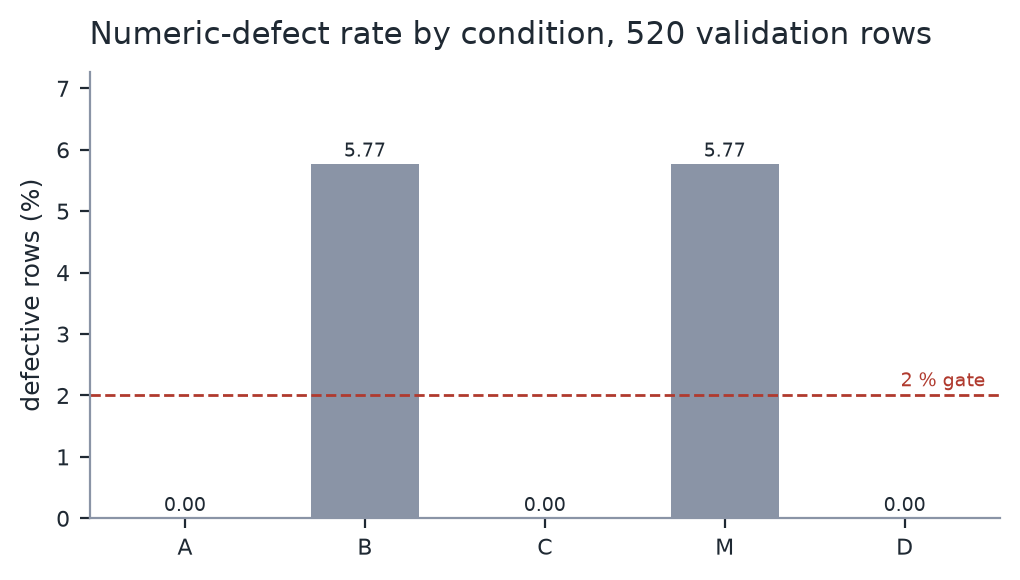
\includegraphics[keepaspectratio]{figures/fig1_cells.png}}
\caption{Numeric-defect rate by condition}
\end{figure}

\begin{longtable}[]{@{}lllllll@{}}
\toprule\noalign{}
cell & numeric & rate & grounding & role & contradiction & anchor \\
\midrule\noalign{}
\endhead
\bottomrule\noalign{}
\endlastfoot
A & \textbf{0} & 0.00 \% & 0 & 0 & 0 & \textbf{520/520} \\
B & 30 & 5.77 \% & 33 & 57 & 0 & 188/520 \\
C & \textbf{0} & 0.00 \% & 1 & 17 & 0 & \textbf{520/520} \\
M & 30 & 5.77 \% & 32 & 43 & 0 & 191/520 \\
D & 0 & 0.00 \% & 0 & 0 & 0 & 262/520 \\
\end{longtable}

McNemar, B against A: 30 versus 0, exact p =
\(2 \cdot 0.5^{30} \approx 1.9 \times 10^{-9}\) (the scorer's stored
field reads 0.0, a float underflow, so the value is derived from the
discordant counts). The seams certify: C leaks 0 of B's numeric values
and M leaks 0 of A's. D substitutes A on 114 of 520 rows (21.9 \%),
inside its pre-registered 25 \% ceiling; the signed decision records
that figure as ``A with extra steps'' rather than a certified pass,
because the 27.3 \% rate it was signed against predates two checker
corrections.

Note what the cell table does not show: B's numeric rate (5.77 \%) is
the highest in the table, but C --- A's numbers inside B's prose --- is
exact. The numbers, not the prose, carry the defect.

\subsubsection{6.2 Confirmatory pass}\label{confirmatory-pass}

\begin{figure}
\centering
\pandocbounded{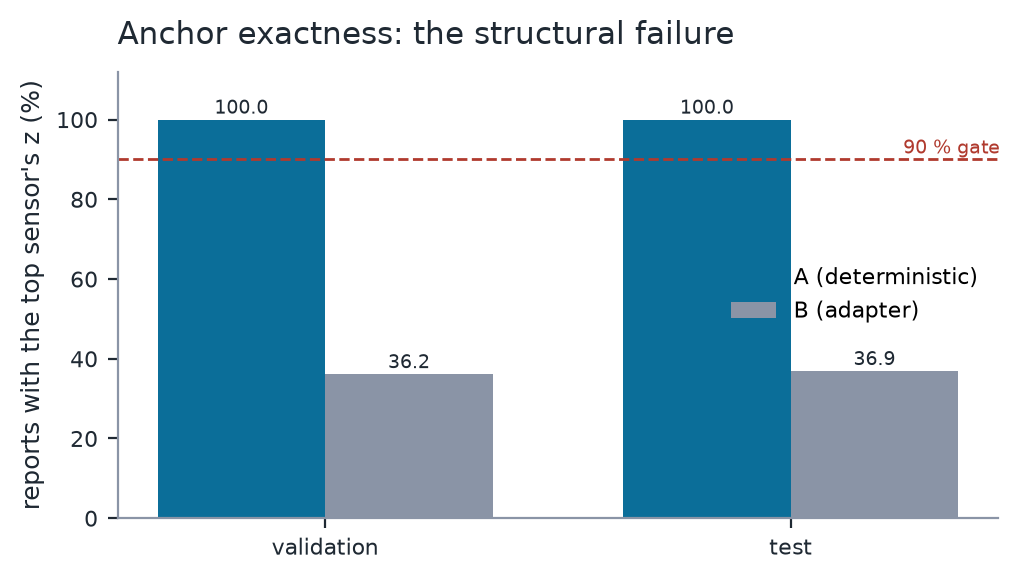
\includegraphics[keepaspectratio]{figures/fig4_anchor.png}}
\caption{Anchor exactness}
\end{figure}

\begin{longtable}[]{@{}
  >{\raggedright\arraybackslash}p{(\linewidth - 8\tabcolsep) * \real{0.2000}}
  >{\raggedright\arraybackslash}p{(\linewidth - 8\tabcolsep) * \real{0.2000}}
  >{\raggedright\arraybackslash}p{(\linewidth - 8\tabcolsep) * \real{0.2000}}
  >{\raggedright\arraybackslash}p{(\linewidth - 8\tabcolsep) * \real{0.2000}}
  >{\raggedright\arraybackslash}p{(\linewidth - 8\tabcolsep) * \real{0.2000}}@{}}
\toprule\noalign{}
\begin{minipage}[b]{\linewidth}\raggedright
check
\end{minipage} & \begin{minipage}[b]{\linewidth}\raggedright
A
\end{minipage} & \begin{minipage}[b]{\linewidth}\raggedright
B
\end{minipage} & \begin{minipage}[b]{\linewidth}\raggedright
gate
\end{minipage} & \begin{minipage}[b]{\linewidth}\raggedright
verdict
\end{minipage} \\
\midrule\noalign{}
\endhead
\bottomrule\noalign{}
\endlastfoot
numeric & \textbf{0 (0.00 \%)} & \textbf{40 (1.26 \%)} & $\leq$ 2 \% & both
pass \\
grounding & 250 (7.89 \%) & 325 (10.26 \%) & $\leq$ 2 \% & both fail \\
contradiction & 0 & 5 (0.16 \%) & $\leq$ 2 \% & both pass \\
instrument role & 0 & 458 (14.46 \%) & $\leq$ 2 \% & B fails \\
anchor exact & \textbf{3,168 (100 \%)} & \textbf{1,170 (36.93 \%)} & $\geq$
90 \% & B fails \\
\end{longtable}

McNemar: 40 versus 0, exact p =
\(2 \cdot 0.5^{40} \approx 1.8 \times 10^{-12}\) (stored as 0.0 by
underflow, derived from the counts). B's anchor failures decompose into
an omitted z-score (1,459 rows, 46.05 \%), a value contradicting the
stored one (203, 6.41 \%), and a named sensor that was never on the page
(336, 10.61 \%).

This is the paper's central contrast. The adapter meets the numeric
budget on held-out data --- a genuinely good result for a 2B model
writing technical prose --- and simultaneously fails every structural
check, by margins no reviewer would call marginal.

\subsubsection{6.3 Where the numeric defects actually
are}\label{where-the-numeric-defects-actually-are}

\begin{figure}
\centering
\pandocbounded{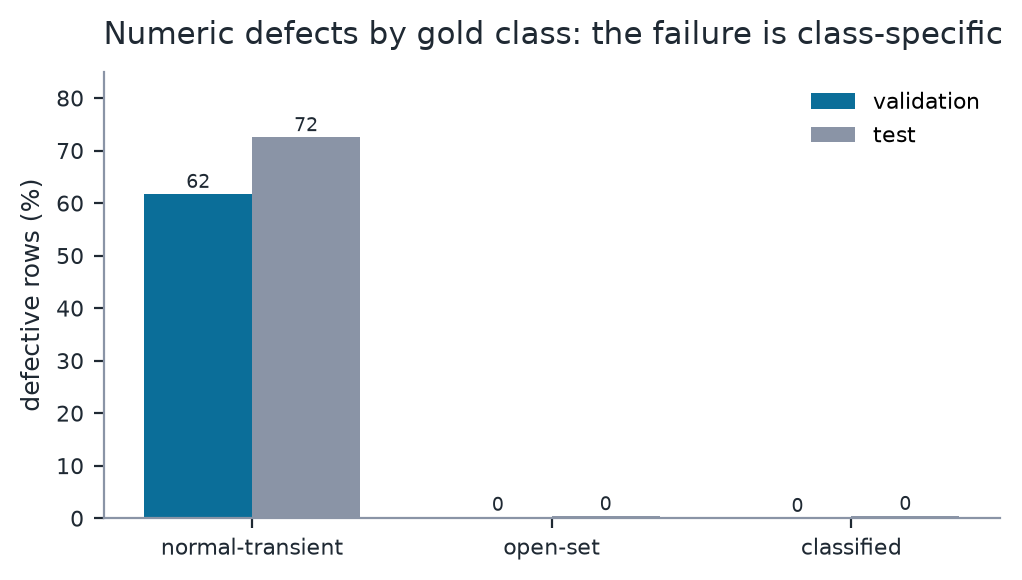
\includegraphics[keepaspectratio]{figures/fig2_stratified.png}}
\caption{Defects by gold class}
\end{figure}

\begin{longtable}[]{@{}lll@{}}
\toprule\noalign{}
gold class & fit set & confirmatory \\
\midrule\noalign{}
\endhead
\bottomrule\noalign{}
\endlastfoot
normal-transient & \textbf{29/47 = 61.7 \%} & \textbf{29/40 = 72.5
\%} \\
open-set & 1/454 = 0.2 \% & 6/1,814 = 0.3 \% \\
classified & 0/19 = 0 \% & 5/1,314 = 0.4 \% \\
\end{longtable}

The unstratified rates (5.77 \% versus 1.26 \%) differ by 4.6$\times$, and the
gap is almost entirely composition: the only class where the writer
fails is 9.0 \% of the fit set and 1.3 \% of the confirmatory pass.
Within the failing class the counts are nearly identical (29 and 29). An
earlier draft of this work read the unstratified gap as split
dependence; stratifying dissolves it.

The two splits were rendered from slightly different prompt builds (\S8),
so we claim consistency across two builds, not stability across
identical conditions: in both, the defect concentrates on no-alarm
narratives and is near-absent elsewhere. The matched counts do not
depend on the template difference, and the comparison is within class
throughout.

The failure mode is specific and reproducible: writing a no-alarm
narrative, the adapter attaches inequality claims to detectors whose
stored values point the other way. That is an error a deployment can
monitor for directly (count inequality claims in normal-transient
reports), which is more useful than a global defect rate.

\subsubsection{6.4 Diagnosis channel}\label{diagnosis-channel}

\begin{figure}
\centering
\pandocbounded{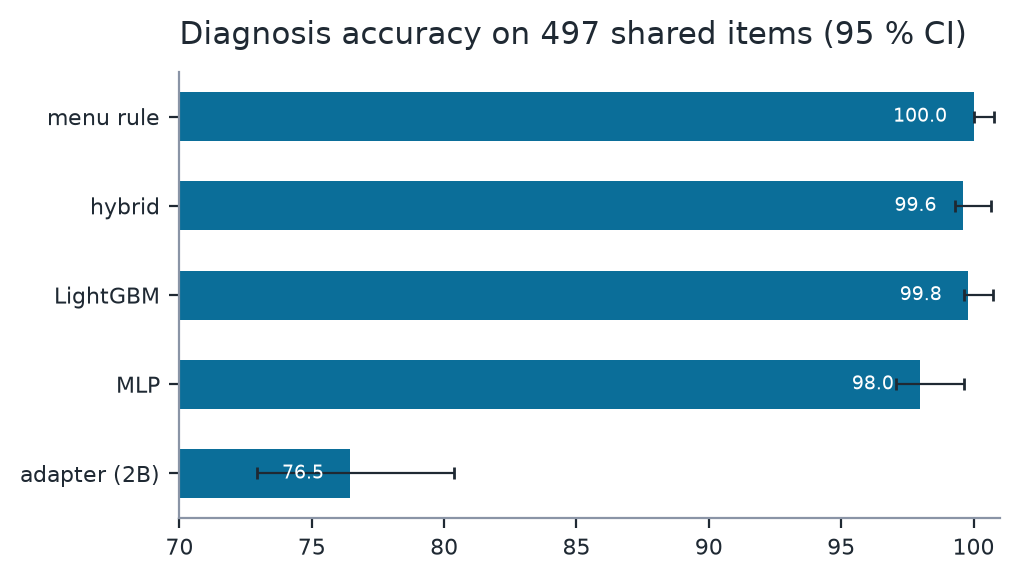
\includegraphics[keepaspectratio]{figures/fig3_classifier.png}}
\caption{Diagnosis accuracy}
\end{figure}

On the 497 items where all systems produce a label:

\begin{longtable}[]{@{}lll@{}}
\toprule\noalign{}
system & accuracy & 95 \% CI \\
\midrule\noalign{}
\endhead
\bottomrule\noalign{}
\endlastfoot
menu rule & 1.0000 & 0.9923--1.0000 \\
hybrid (shipped) & 0.9960 & 0.9854--0.9989 \\
LightGBM & 0.9980 & 0.9887--0.9996 \\
MLP & 0.9799 & 0.9634--0.9890 \\
adapter alone & 0.8330 & 0.7977--0.8632 \\
\end{longtable}

The ``adapter alone'' row is the protocolA adapter at checkpoint 300,
the checkpoint the macro-F1 selection chose; it is not the adapter named
in the deployment configuration, which is a different set of weights and
is not scored in this comparison.

Hybrid against LightGBM: 2 versus 1 discordant (b = 2, c = 1), exact p =
1.0. The knowledge-base layer buys no accuracy, and the adapter as a
classifier is clearly behind --- against the hybrid the adapter loses 1
versus 82, of which 43 are open-set items the hybrid correctly declined.
The layer's justification must therefore be explanatory coverage and
dialogue grounding, which we do not claim to have measured as a
preference.

\textbf{Re-measured 2026-11-16, after the feature-vocabulary fix.} The
classifier's columns named the manipulated variables \texttt{XMV\_1..11}
while the evidence page prints \texttt{XMV\_42..52}, so 22.4 \% of the
sensors listed on stored pages had no column and contributed nothing.
With the vocabulary aligned and every classifier-side model retrained,
the table above replaces the earlier menu rule 0.9980, hybrid 0.9940,
LightGBM 0.9940 and MLP 0.9698. The adapter row is unchanged: its
predictions never depended on those features. On the cross-fitted
evaluation the same fix moves observable accuracy from 0.9781 to 0.9878
and macro-F1 from 0.9708 to 0.9843, so the paper's diagnosis numbers are
the post-fix ones.

\subsubsection{6.5 Preference}\label{preference}

\begin{longtable}[]{@{}lll@{}}
\toprule\noalign{}
pairing & rater 1 & rater 2 \\
\midrule\noalign{}
\endhead
\bottomrule\noalign{}
\endlastfoot
A versus C & 98 / 20 & 70 / 48 \\
B versus C & 10 / 108 & 53 / 64 \\
B versus M & 0 / 114 & 2 / 112 \\
\end{longtable}

360 pairs, two readers: observed agreement 0.7778, expected 0.4739,
Cohen's kappa 0.5776 --- below the declared 0.60 floor, so the
preference tier is reported descriptively and supports no claim.
Publishing a preference ordering at this reliability would be the exact
error that judge-noise work warns about \citep{zheng2023judging}. The
three contrast orders above are quoted only because the signed decision
requires them to be visible, not as evidence of ordering.

\subsubsection{6.6 Selection}\label{selection}

A six-rung selector applies pre-registered rungs in order. Rung 1 vetoes
B (5.77 \% against a 1.00 \% ceiling set as A + 1 pp). Rungs 2--4 are
unavailable: preference is below its floor, and no eligible passer
carries an independently verified mechanism claim. Rung 5 compares time
per 520-row pass on a pre-signed cost basis; A and D tie, and the
declared tie-break selects A. The resulting receipt
(\texttt{decided\_by\_rung\ 5}, chosen A) is committed with the paper,
and no dollar figure is claimed.

D is a legitimate engineering option and it does not lose on any
measured axis --- it simply contributes nothing of its own on the 21.9
\% of rows where it substitutes.

\subsection{7. Discussion}\label{discussion}

\textbf{What the separation buys.} A label that is auditable, calibrated
and refusal-capable; prose that cannot launder a wrong diagnosis into an
authoritative-looking report; a system that keeps reporting when the
classifier, the guard or the adapter fails.

\textbf{What it costs.} The classifier is the accuracy ceiling (LightGBM
alone matches it); the threshold is nearly inert because calibration
saturates (98.3 \% of calibrated maxima equal the threshold); lookalike
faults absorb each other; and open-set refusal, while correct, is what
most of the remaining error consists of.

\textbf{Why structure, not numbers, is the right axis.} A numeric budget
of 2 \% is met by this adapter, and a reader who stopped there would
conclude the writer is safe. The structural checks show the opposite:
the same reports drop the anchor, misbind roles and cite absent tags.
Structural fidelity is cheap to check, hard to satisfy accidentally, and
closer to what an auditor actually reads for.

\subsection{8. Threats to validity and
limitations}\label{threats-to-validity-and-limitations}

\begin{enumerate}
\def\labelenumi{\arabic{enumi}.}
\tightlist
\item
  \textbf{Template drift between splits.} The stored fit-set prompts
  were generated under an earlier prompt build (0 of 520 match the
  current builder byte-for-byte). All cross-split comparisons are
  therefore within class, and \S6.3 is the only cross-split claim we
  make.
\item
  \textbf{One adapter configuration.} Seed 42, one order on the
  confirmatory pass, greedy decoding. Batch size is a measurement
  parameter, not a neutral setting: only 1 of 12 texts was identical
  between batch 16 and batch 8. Order invariance was measured on the fit
  set only (368/520 identical defect profiles, 0.7077); the test split
  was run on the kb order alone.
\item
  \textbf{Saturation.} 98.3 \% of calibrated maxima equal the threshold,
  so threshold choice barely moves decisions; the abstention numbers are
  therefore a property of the calibration, not of a tuned operating
  point.
\item
  \textbf{D's ceiling.} D's substitution rate is inside its 25 \%
  ceiling on the corrected instrument (21.9 \%), while the signed
  decision predates the correction. We describe D conservatively as A
  with extra steps rather than claim a certified pass.
\item
  \textbf{Live accuracy is not estimated here.} The stored event archive
  predates run provenance and cannot be resolved to simulator truth.
  Events now carry source file, simulation run and fault number, so a
  replay or simulator-fed deployment is scorable, but no such run is
  reported in this paper.
\item
  \textbf{Unobservable faults.} Faults 3 and 9 are predicted
  NORMAL\_TRANSIENT at confidence 1.0; they are unobservable in this
  dataset, and the menu excludes them.
\item
  \textbf{Not measured.} Detector frontier, follow-up dialogue
  condition, cross-path parity of the two scoring implementations, and
  any latency claim other than the generator's. Each is listed as future
  work rather than estimated.
\end{enumerate}

\subsection{9. Reproducibility and
evidence}\label{reproducibility-and-evidence}

Every number source cited above is committed in
\texttt{docs/\allowbreak{}reports/\allowbreak{}evidence/\allowbreak{}} as a byte-identical copy with a SHA-256
hash, because the working artefacts live in an untracked
\texttt{outputs/\allowbreak{}} tree. Appendix A maps each claim to its file;
\texttt{docs/\allowbreak{}reports/\allowbreak{}evidence/\allowbreak{}index.json} carries the full hashes, and
\texttt{scripts/\allowbreak{}bundle\_\allowbreak{}evidence.py\ -\/\allowbreak{}-check} fails if a copy or an
origin has drifted.

\begin{longtable}[]{@{}
  >{\raggedright\arraybackslash}p{(\linewidth - 4\tabcolsep) * \real{0.3333}}
  >{\raggedright\arraybackslash}p{(\linewidth - 4\tabcolsep) * \real{0.3333}}
  >{\raggedright\arraybackslash}p{(\linewidth - 4\tabcolsep) * \real{0.3333}}@{}}
\toprule\noalign{}
\begin{minipage}[b]{\linewidth}\raggedright
artefact
\end{minipage} & \begin{minipage}[b]{\linewidth}\raggedright
role
\end{minipage} & \begin{minipage}[b]{\linewidth}\raggedright
SHA-256 (first 16)
\end{minipage} \\
\midrule\noalign{}
\endhead
\bottomrule\noalign{}
\endlastfoot
\texttt{n4\_cells.json} & fit-set cells, seams, D fallback, McNemar &
\texttt{5a9392ff5399785f} \\
\texttt{test\_contrast.json} & confirmatory counts, rates, anchors &
\texttt{9de4c06656d57fbf} \\
\texttt{classifier\_contrasts.json} & diagnosis table, CIs, discordants
& \texttt{2c91b6f626abec16} \\
\texttt{order\_invariance.json} & 368/520 across prompt orders &
\texttt{40da08c93c9c01c8} \\
\texttt{preference\_result.json} & 360 pairs, both raters &
\texttt{0f1f463e373b0690} \\
\texttt{preference\_kappa.json} & kappa and disagreements &
\texttt{bdb8792bf49abcc1} \\
\texttt{selection\_receipt.json} & rung-5 receipt &
\texttt{0bd8ed9c0f39839f} \\
\texttt{d\_ceiling\_decision.json} & signed D decision &
\texttt{d57cdcfd7c92bb1b} \\
\texttt{cases46\_audit.csv} & 46/46 calibration &
\texttt{fbb0044d8ac0f939} \\
\end{longtable}

Figures are rendered from stored JSON: \texttt{figure\_data.json} feeds
figures 1--3 and the anchor figure reads the same cell and test
summaries as the tables. Two audit scripts accompany the paper:
\texttt{verify\_paper\_numbers.py} re-derives every table and inspects
the built PDF (104 checks), and \texttt{audit\_claim\_sheets.py}
recomputes the claims registry and resolves every cited path (74
checks).

\subsection{10. Conclusion}\label{conclusion}

A 2B adapter can write industrial fault reports that stay inside a
numeric-fidelity budget on held-out data, and it will still fail the
checks that decide whether an operator can trust a paragraph: it will
drop the top sensor's z-score, call a detector an actuator, and mention
a tag that was never on the page. The failures are concentrated,
monitorable and class-specific rather than diffuse. Keep the diagnosis
deterministic, measure structure as carefully as you measure numbers,
and report stratified rates --- an unstratified rate hid both the size
and the shape of the adapter's defect for several revisions of this
work.

\subsection{Data availability}\label{data-availability}

All numbers are reproduced from the artefacts in
\texttt{docs/\allowbreak{}reports/\allowbreak{}evidence/\allowbreak{}} at the commit that carries this paper.
The underlying plant simulations are the public Tennessee Eastman
benchmark; prompt and generation text is not redistributed. Code for the
checks, the figures and the paper build is in \texttt{scripts/\allowbreak{}}.

\subsection{Appendix A. Claim to evidence
map}\label{appendix-a.-claim-to-evidence-map}

\begin{longtable}[]{@{}
  >{\raggedright\arraybackslash}p{(\linewidth - 4\tabcolsep) * \real{0.3333}}
  >{\raggedright\arraybackslash}p{(\linewidth - 4\tabcolsep) * \real{0.3333}}
  >{\raggedright\arraybackslash}p{(\linewidth - 4\tabcolsep) * \real{0.3333}}@{}}
\toprule\noalign{}
\begin{minipage}[b]{\linewidth}\raggedright
claim
\end{minipage} & \begin{minipage}[b]{\linewidth}\raggedright
statement
\end{minipage} & \begin{minipage}[b]{\linewidth}\raggedright
evidence file
\end{minipage} \\
\midrule\noalign{}
\endhead
\bottomrule\noalign{}
\endlastfoot
C1 & the deterministic writer carries no numeric-defect liability; the
adapter's small one meets budget (0/3,168 versus 40/3,168 = 1.26 \%) &
\texttt{n4\_cells.json}, \texttt{test\_contrast.json},
\texttt{order\_invariance.json} \\
C2 & anchor exactness is where the writer fails structurally
(1,170/3,168 = 36.93 \%; z omitted 46.05 \%) & \texttt{n4\_cells.json}
anchor\_exact, \texttt{test\_contrast.json} anchor\_status \\
C3 & a plain gradient-boosted classifier matches the calibrated hybrid
(0.9980 versus 0.9960, 2 versus 1, p = 1) &
\texttt{classifier\_contrasts.json}, \texttt{adapter\_summary.json},
\texttt{preds\_val\_full\_300.jsonl} \\
C4 & pairwise preference cannot carry a claim (kappa 0.5776 over 360
pairs) & \texttt{preference\_result.json},
\texttt{preference\_kappa.json} \\
C5 & selection is decided on cost at rung 5, not on quality &
\texttt{selection\_receipt.json} \\
C6 & the fallback wrapper stays inside budget (114/520 = 21.9 \%) under
the signed conservative framing & \texttt{n4\_cells.json} seam
certification, \texttt{d\_ceiling\_decision.json} \\
instrument & the contradiction checker agrees with all 46 hand-written
cases & \texttt{cases46\_audit.csv} \\
\end{longtable}

\subsection{Non-claims}\label{non-claims}

No claim that the adapter is more faithful than the deterministic
writer; no cross-split rate comparison; no preference ordering; no
mechanism-quality claim; no latency claim outside the generator; no
detector-frontier comparison; no live-accuracy estimate.

\bibliography{references.bib}

\end{document}
